\documentclass{beamer}
\usepackage[utf8]{inputenc}

\usetheme{Madrid}
\usecolortheme{default}
\usepackage{amsmath,amssymb,amsfonts,amsthm}
\usepackage{mathtools}
\usepackage{txfonts}
\usepackage{tkz-euclide}
\usepackage{listings}
\usepackage{adjustbox}
\usepackage{array}
\usepackage{gensymb}
\usepackage{tabularx}
\usepackage{gvv}
\usepackage{lmodern}
\usepackage{circuitikz}
\usepackage{tikz}
\lstset{literate={·}{{$\cdot$}}1 {λ}{{$\lambda$}}1 {→}{{$\to$}}1}
\usepackage{graphicx}

\setbeamertemplate{page number in head/foot}[totalframenumber]

\usepackage{tcolorbox}
\tcbuselibrary{minted,breakable,xparse,skins}



\definecolor{bg}{gray}{0.95}
\DeclareTCBListing{mintedbox}{O{}m!O{}}{%
  breakable=true,
  listing engine=minted,
  listing only,
  minted language=#2,
  minted style=default,
  minted options={%
    linenos,
    gobble=0,
    breaklines=true,
    breakafter=,,
    fontsize=\small,
    numbersep=8pt,
    #1},
  boxsep=0pt,
  left skip=0pt,
  right skip=0pt,
  left=25pt,
  right=0pt,
  top=3pt,
  bottom=3pt,
  arc=5pt,
  leftrule=0pt,
  rightrule=0pt,
  bottomrule=2pt,
  toprule=2pt,
  colback=bg,
  colframe=orange!70,
  enhanced,
  overlay={%
    \begin{tcbclipinterior}
    \fill[orange!20!white] (frame.south west) rectangle ([xshift=20pt]frame.north west);
    \end{tcbclipinterior}},
  #3,
}
\lstset{
    language=C,
    basicstyle=\ttfamily\small,
    keywordstyle=\color{blue},
    stringstyle=\color{orange},
    commentstyle=\color{green!60!black},
    numbers=left,
    numberstyle=\tiny\color{gray},
    breaklines=true,
    showstringspaces=false,
}
%------------------------------------------------------------
%This block of code defines the information to appear in the
%Title page
\title %optional
{4.11.4}
\date{August 31,2025}
%\subtitle{A short story}

\author % (optional)
{Harsha-EE25BTECH11026}



\begin{document}


\frame{\titlepage}


\begin{frame}{Question}
Find the equation of the plane which contains the line of intersection of the planes $\vec{r}.\brak{\hat{i}+2\hat{j}+3\hat{k}}-4=0$ and $\vec{r}.\brak{2\hat{i}+\hat{j}-\hat{k}}+5=0$ and which is perpendicular to the plane $\vec{r}.\brak{5\hat{i}+3\hat{j}-6\hat{k}}+8=0$.
\end{frame}

\begin{frame}{Theoretical Solution}
According to the question,\\
\begin{align}
    \vec{n_1}=\myvec{1\\2\\3} \quad \vec{n_2}=\myvec{2\\1\\-1} \quad c_1=4 \quad c_2=-5
\end{align}
\end{frame}

\begin{frame}{Equation}
The equation of intersection of planes is given by
\begin{align}
    \vec{n_1}^{\top}\vec{x}-c_1+\lambda\brak{\vec{n_2}^{\top}\vec{x}-c_2}=0
\end{align}
\begin{align}
    \implies \brak{\vec{n_1}^{\top}+\lambda\vec{n_2}^{\top}}\vec{x}=c_1+\lambda c_2
\end{align}
\end{frame}

\begin{frame}{Theoretical Solution}
Let the direction vector of the plane perpendicular to intersection of planes be $\vec{n_3}$
\begin{align}
    \therefore \brak{\vec{n_1}^{\top}+\lambda\vec{n_2}^{\top}}\vec{n_3}=0
\end{align}
\begin{align}
    \implies \lambda=-\frac{\vec{n_1}^{\top}\vec{n_3}}{\vec{n_2}^{\top}\vec{n_3}}
\end{align}
\end{frame}
\begin{frame}{Theoretical Solution}
\begin{align}
    \therefore \lambda=-\frac{\myvec{1&&2&&3}\myvec{5\\3\\-6}}{\myvec{2&&1&&-1}\myvec{5\\3\\-6}}=\frac{7}{19}
\end{align}
\begin{align}
    \implies \text{equation of the plane\,:\;} \myvec{33&&45&&50}\vec{x}=41
\end{align}
\end{frame}

\begin{frame}[fragile]
    \frametitle{C Code -Finding Equation of the plane}

    \begin{lstlisting}
#include <stdio.h>
// Function to compute required plane coefficients
void required_plane(double n1[3], double d1,
                    double n2[3], double d2,
                    double n3[3], double d3,
                    double n_req[3], double *d_req) {
    
    // Find λ such that (n1 + λn2)·n3 = 0
    double dot_n1n3 = n1[0]*n3[0] + n1[1]*n3[1] + n1[2]*n3[2];
    double dot_n2n3 = n2[0]*n3[0] + n2[1]*n3[1] + n2[2]*n3[2];
    double lam = -dot_n1n3 / dot_n2n3;
    // Required normal = n1 + λ n2
    for(int i=0; i<3; i++) {
        n_req[i] = n1[i] + lam * n2[i];
    }
    // Required constant term
    *d_req = d1 + lam * d2;
}

    \end{lstlisting}
\end{frame}

\begin{frame}[fragile]
    \frametitle{Python+C code}

    \begin{lstlisting}[language=Python]
import ctypes
import numpy as np
import sympy as sp
import matplotlib.pyplot as plt
import matplotlib as mp
from fractions import Fraction
import math
mp.use("TkAgg")

lib = ctypes.CDLL("./libplane.so")
# Define argtypes and restype
lib.required_plane.argtypes = [
    ctypes.POINTER(ctypes.c_double), ctypes.c_double,
    ctypes.POINTER(ctypes.c_double), ctypes.c_double,
    ctypes.POINTER(ctypes.c_double), ctypes.c_double,
    ctypes.POINTER(ctypes.c_double), ctypes.POINTER(ctypes.c_double)]
lib.required_plane.restype = None

    \end{lstlisting}
\end{frame}

\begin{frame}[fragile]
    \frametitle{Python+C code}

    \begin{lstlisting}[language=Python]
# Input planes
n1 = (ctypes.c_double * 3)(1, 2, 3)
d1 = -4.0
n2 = (ctypes.c_double * 3)(2, 1, -1)
d2 = 5.0
n3 = (ctypes.c_double * 3)(5, 3, -6)
d3 = 8.0
# Output storage
n_req = (ctypes.c_double * 3)()
d_req = ctypes.c_double()
# Call C function
lib.required_plane(n1, d1, n2, d2, n3, d3, n_req, ctypes.byref(d_req))
# Convert to numpy + sympy
n_req_np = np.array([n_req[i] for i in range(3)], dtype=float)
d_req_val = float(d_req.value)
n_vec = sp.Matrix(n_req_np)

    \end{lstlisting}
\end{frame}

\begin{frame}[fragile]
    \frametitle{Python+C code}

    \begin{lstlisting}[language=Python]
# Formatting helpers
def format_plane_integer(n, d):
    # Fractions for exactness
    n_frac = [Fraction(str(float(v))).limit_denominator() for v in n]
    d_frac = Fraction(str(float(d))).limit_denominator()
    # LCM of denominators
    denoms = [f.denominator for f in n_frac] + [d_frac.denominator]
    lcm = math.lcm(*denoms)
    n_int = [int(f * lcm) for f in n_frac]
    d_int = int(d_frac * lcm)
    # Fix sign convention 
    # Equation is n·r + d = 0  →  n·r = -d
    rhs = -d_int

    \end{lstlisting}
\end{frame}

\begin{frame}[fragile]
    \frametitle{Python+C code}

    \begin{lstlisting}[language=Python]
# Make gcd simplification
g = math.gcd(math.gcd(abs(n_int[0]), abs(n_int[1])), math.gcd(abs(n_int[2]), abs(rhs)))
n_int = [ni // g for ni in n_int]
rhs //= g
return f"r · ({n_int[0]}, {n_int[1]}, {n_int[2]}) = {rhs}"
x, y, z = sp.symbols('x y z')
plane_eq = n_vec[0]*x + n_vec[1]*y + n_vec[2]*z + d_req_val
print("\nEquation of required plane:")
print(format_plane_integer(n_req_np, d_req_val))
    \end{lstlisting}
    
\end{frame}

\begin{frame}[fragile]
    \frametitle{Python+C code}

    \begin{lstlisting}[language=Python]
# Step 6: Plot planes
fig = plt.figure(figsize=(8,8))
ax = fig.add_subplot(111, projection='3d')

def plot_plane(ax, n, d, color, alpha=0.4):
    xx, yy = np.meshgrid(np.linspace(-5,5,15), np.linspace(-5,5,15))
    zz = (-n[0]*xx - n[1]*yy - d) / n[2]
    ax.plot_surface(xx, yy, zz, color=color, alpha=alpha)
    
# Convert sympy / ctypes → float numpy
n1f, d1f = np.array([1,2,3], dtype=float), -4.0
n2f, d2f = np.array([2,1,-1], dtype=float), 5.0
n3f, d3f = np.array([5,3,-6], dtype=float), 8.0
nrf = n_req_np
drf = d_req_val


    \end{lstlisting}
    
\end{frame}

\begin{frame}[fragile]
    \frametitle{Python+C code}

    \begin{lstlisting}[language=Python]

# Plot given planes and required plane
plot_plane(ax, n1f, d1f, "red", 0.2)     # π1
plot_plane(ax, n2f, d2f, "blue", 0.2)    # π2
plot_plane(ax, n3f, d3f, "green", 0.2)   # π3
plot_plane(ax, nrf, drf, "purple", 0.6)  # Required plane

ax.set_xlabel("X")
ax.set_ylabel("Y")
ax.set_zlabel("Z")
ax.set_title(r"Required Plane through Intersection, $\perp$ to Given Plane")

plt.savefig("/home/user/Matrix/Matgeo_assignments/4.11.4/figs/Figure_1", dpi=300, bbox_inches="tight")
plt.show()
    \end{lstlisting}
    
\end{frame}

\begin{frame}[fragile]
    \frametitle{Python code}

    \begin{lstlisting}[language=Python]
import sympy as sp
import numpy as np
import matplotlib.pyplot as plt
import matplotlib as mp
mp.use("TkAgg")
# Step 1: Define symbols
lam = sp.symbols('lam')
# Given plane normals and constants
n1, d1 = sp.Matrix([1,2,3]), -4
n2, d2 = sp.Matrix([2,1,-1]), 5
n3, d3 = sp.Matrix([5,3,-6]), 8
# Step 2: General plane through intersection
n = n1 + lam*n2       # normal vector depends on λ
d = d1 + lam*d2       # constant term
# Step 3: Perpendicular condition
eq = sp.Eq(n.dot(n3), 0)
lam_val = sp.solve(eq, lam)[0]
    \end{lstlisting}
    
\end{frame}

\begin{frame}[fragile]
    \frametitle{Python code}

    \begin{lstlisting}[language=Python]
# Substitute λ into plane equation
n_req = (n.subs(lam, lam_val))
d_req = d.subs(lam, lam_val)

# Step 4: Scale to integers (fix applied here)
all_vals = list(n_req) + [d_req]   # avoid .tolist()
mult = sp.lcm([sp.denom(val) for val in all_vals])
n_req = (n_req * mult).applyfunc(sp.simplify)
d_req = sp.simplify(d_req * mult)

# Step 5: Vector form
x, y, z = sp.symbols('x y z')
plane_eq = n_req[0]*x + n_req[1]*y + n_req[2]*z + d_req
point_on_plane = sp.solve(plane_eq.subs({y:0, z:0}), x)
    \end{lstlisting}
    
\end{frame}

\begin{frame}[fragile]
    \frametitle{Python code}

    \begin{lstlisting}[language=Python]
# Step 6: Plot planes
fig = plt.figure(figsize=(8,8))
ax = fig.add_subplot(111, projection='3d')
def plot_plane(ax, n, d, color, alpha=0.4):
    xx, yy = np.meshgrid(np.linspace(-5,5,15), np.linspace(-5,5,15))
    zz = (-n[0]*xx - n[1]*yy - d) / n[2]
    ax.plot_surface(xx, yy, zz, color=color, alpha=alpha)
# Convert sympy → float numpy
n1f, d1f = np.array(n1, dtype=float), float(d1)
n2f, d2f = np.array(n2, dtype=float), float(d2)
n3f, d3f = np.array(n3, dtype=float), float(d3)
nrf, drf = np.array([float(v) for v in n_req]), float(d_req)
# Plot given planes and required plane
plot_plane(ax, n1f, d1f, "red", 0.2)     
plot_plane(ax, n2f, d2f, "blue", 0.2)    
plot_plane(ax, n3f, d3f, "green", 0.2)   
plot_plane(ax, nrf, drf, "purple", 0.6)  # Required plane
    \end{lstlisting}
    
\end{frame}

\begin{frame}[fragile]
    \frametitle{Python code}

    \begin{lstlisting}[language=Python]
ax.set_xlabel("X")
ax.set_ylabel("Y")
ax.set_zlabel("Z")
ax.set_title(r"Required Plane through Intersection, $\perp$ to Given Plane")
plt.savefig("/home/user/Matrix/Matgeo_assignments/4.11.4/figs/Figure_1")
plt.show()

    \end{lstlisting}
    
\end{frame}

\begin{frame}{Plot}
    \begin{figure}[H]
    \centering
    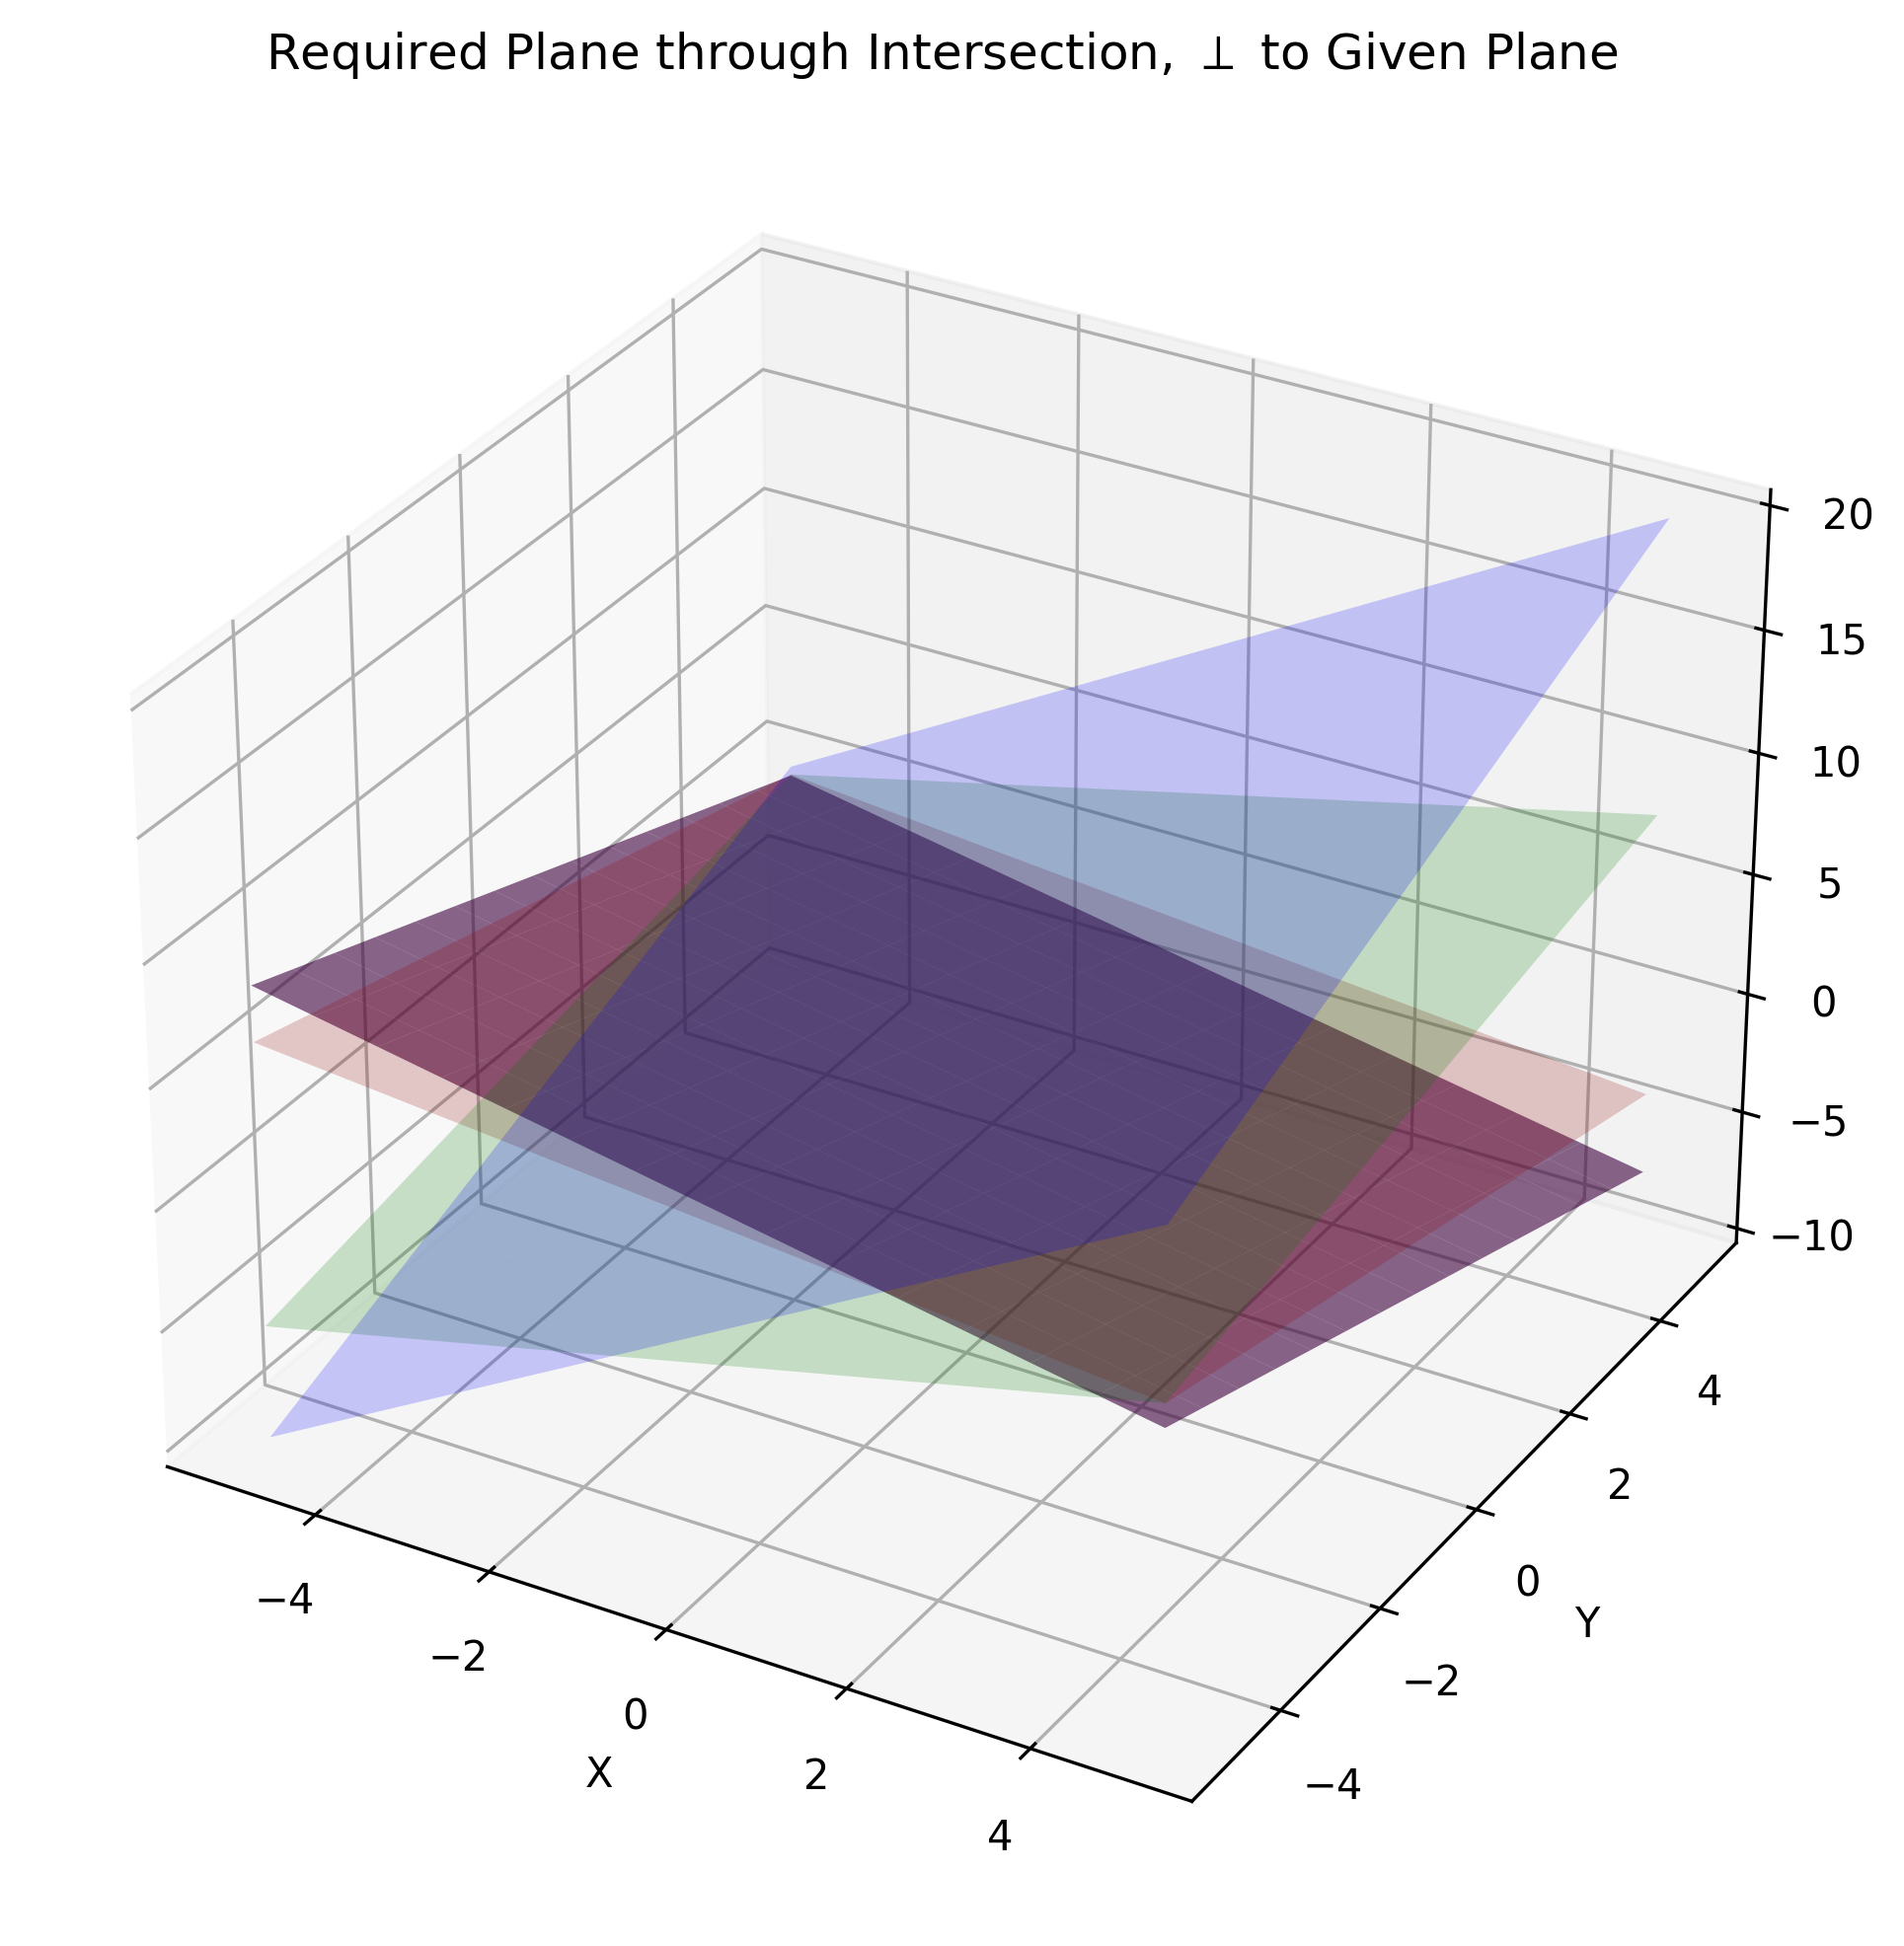
\includegraphics[width=0.6\columnwidth]{figs/Figure_1.png}
    \label{fig:1}
\end{figure}
\end{frame}

\end{document}